\section{Measurement Model}
\label{sec:measurement_model}

The CSQMI of a single beam \eqref{eq:single_beam} depends on the ability
to estimate $p(e_j)$, the probability that the $j$th cell in a raycast is
the first occupied grid cell. Rather than building a measurement model using the
maximum likelihood estimate of $z_{j}$ \cite{charrow15,
thrun2005probabilistic, julian2013mutual}, we compute a discrete distribution over the
raycast, where each cell value directly approximates the probability that cell $c^i$ is the
first occupied cell in $c$, $p(e_j = c^i) \ \forall\ c^{i} \in c$ using the
continuous occupancy values in $c$.

To calculate this distribution, we use a generalization of the geometric
distribution, which is commonly used to determine the number of Bernoulli trials necessary to obtain one success, supported
on the set $\mbb{N}^{+}$. Since each occupancy grid cell in a raycast contains
continuous probabilities $\in [0, 1]$ of the cell's occupancy, we build on the
geometric distribution to support independent, but not identically distributed
(i.n.i.d.) random variables. Using this generalization, the probability that a cell $c^{i}$ terminates the raycast is computed by assuming that the ray passed through all previous cells.
%
\begin{align}
  \begin{split}
    p(e_j = c^{i})
    &=
    o^{i}
    \prod_{j=1}^{i-1}
    (1 - o^{j})
    \label{eq:geometric_brute}
  \end{split}
\end{align}
%
A straightforward implementation can compute \eqref{eq:geometric_brute} in $\mc{O}(C^2)$ operations for all $c^{i} \in c$. However, we were able to derive an efficient recursive formula that runs in $\mc{O}(C)$.
%
\begin{align}
  \begin{split}
    p(e_j = c^{i})
    &=
    o^{i}
    \prod_{j=1}^{i-1}
    (1 - o^{j}) \\
    &=
    o^{i}
    \left(
    \frac
    {o^{i-1}}
    {o^{i-1}}
    \right)
    (1 - o^{i-1})
    \prod_{j=1}^{i-2}
    (1 - o^{j}) \\
    &=
    o^{i}
    \frac
    {
      1 - o^{i-1}
    }
    {
      o^{i-1}
    }
    p(e_j = c^{i-1}) \\
    &=
    o^{i}
    \left(
    \frac{1}{o^{i-1}}
      -
      1
    \right)
    p(e_j = c^{i-1})
  \end{split}
\end{align}
%
The distribution $p(e_j)$ is depicted over a one-dimensional raycast in Fig.~\ref{fig:measurement_model}.

\begin{figure}
  \centering
  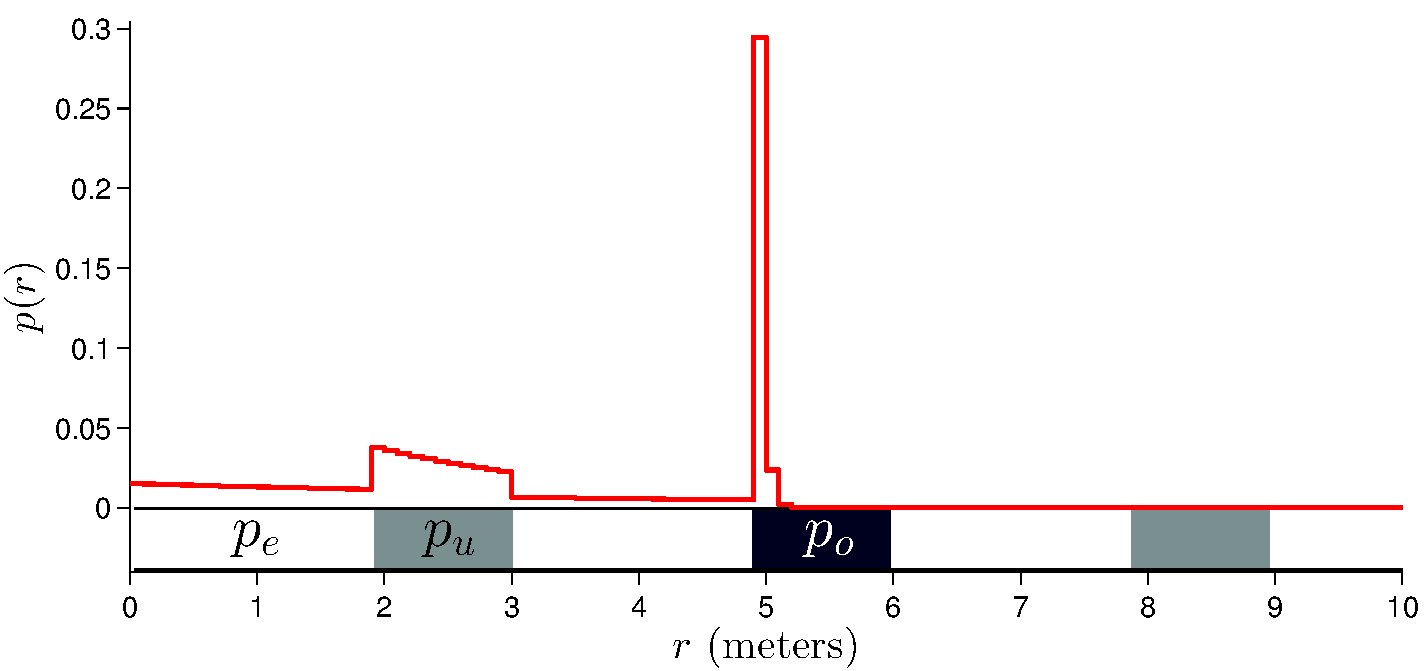
\includegraphics[width=0.5\textwidth]{meas_model.pdf}
  \caption{The distribution $p(e_j)$ over a depicted 1-dimensional map, where $p_{e} = 0.01$, $p_{o} = 0.92$, $p_{u} = 0.05$. \label{fig:measurement_model}}
\end{figure}

